%% $RCSfile: proj_report_outline.tex,v $
%% $Revision: 1.3 $
%% $Date: 2016/06/10 03:41:54 $
%% $Author: kevin $

\documentclass[11pt
              , a4paper
              , twoside
              , openright
              ]{report}


\usepackage{float} % lets you have non-floating floats

\usepackage{url} % for typesetting urls

\usepackage{listings} % for code.

\usepackage{cite}

%
%  We don't want figures to float so we define
%
\newfloat{fig}{thp}{lof}[chapter]
\floatname{fig}{Figure}

%% These are standard LaTeX definitions for the document
%%                            
\title{Whiley to Web Assembly}
\author{Shane Anthony Brewer}


%% This file can be used for creating a wide range of reports
%%  across various Schools
%%
%% Set up some things, mostly for the front page, for your specific document
%
% Current options are:
% [ecs|msor|sms]          Which school you are in.
%                         (msor option retained for reproducing old data)
% [bschonscomp|mcompsci]  Which degree you are doing
%                          You can also specify any other degree by name
%                          (see below)
% [font|image]            Use a font or an image for the VUW logo
%                          The font option will only work on ECS systems
%
\usepackage[image,ecs]{vuwproject}
\otherdegree{Bachelor of Software Engineering with Honours}

% You should specifiy your supervisor here with
%     \supervisor{Firstname Lastname}
% use \supervisors if there is more than one supervisor
\supervisor{Dr David  J. Pearce}
% Unless you've used the bschonscomp or mcompsci
%  options above use
%   \otherdegree{OTHER DEGREE OR DIPLOMA NAME}
% here to specify degree

% Comment this out if you want the date printed.
\date{}

\begin{document}

% Make the page numbering roman, until after the contents, etc.
\frontmatter

%%%%%%%%%%%%%%%%%%%%%%%%%%%%%%%%%%%%%%%%%%%%%%%%%%%%%%%

%%%%%%%%%%%%%%%%%%%%%%%%%%%%%%%%%%%%%%%%%%%%%%%%%%%%%%%

\begin{abstract}

Web Assembly is a new binary language for the web. Its been developed to be a compile target for higher level languages. Whiley can be extend so that it can compile to this new assembly language. Once Whiley is compilable to Web Assembly then the world of the web opens up for programming possibilities.

\end{abstract}

%%%%%%%%%%%%%%%%%%%%%%%%%%%%%%%%%%%%%%%%%%%%%%%%%%%%%%%

\maketitle

\chapter*{Acknowledgments}\label{C:ack} 
I would like to thank David Pearce for the work that he put in as my supervisor. 


\tableofcontents

% we want a list of the figures we defined
\listof{fig}{Figures}

%%%%%%%%%%%%%%%%%%%%%%%%%%%%%%%%%%%%%%%%%%%%%%%%%%%%%%%

\mainmatter

%%%%%%%%%%%%%%%%%%%%%%%%%%%%%%%%%%%%%%%%%%%%%%%%%%%%%%%

% individual chapters included here
\chapter{Introduction}\label{C:intro}

\section{The Context}
Whiley is a programming language that mixes features from object orientated and functional languages. The aim of Whiley is to offer programmers language level code verification. Due to software failures being able to prove aspects of a program are important. This is no less true when developing for the web. With web based applications handling security and monetary transactions. Being able to prove that these types of program are working as intended is important. (Need to add more.)

\section{The Opportunity}
With the introduction of Web Assembly (wasm), a fast efficient binary format for the web, Whiley has a new compile target. Work has been done previously to compile Whiley to both JavaScript and ASM.js. While both languages work on the web, neither are assembly languages. Now Whiley has a language on the web specificity made to be compiled too. (Need to add more.)

\section{Current Status}
The Whiley-to-WebAssembly translator is the step between Whiley's intermediary language (WyIL) and Web Assembly. Currently an WyIL file is passed to an Java implementation of a the translator which then parses it. The parsing creates an absract syntax tree of the file in wasm. That tree can then be written as a wasm file. With that Whiley applications can be run in browsers made by Google, Mozilla, and Microsoft \cite{8_wagner_2016}. To ensure that those files when created run correctly a test harness has been set up. There are 440 test (from the Whiley test suite) that are run, of which 191 pass (Need to change to be more accurate). All the basic types are working along with types like arrays.


\chapter{Background}\label{C:bg}

%%This chapter covers Web Assembly and briefly covers Whiley along with its intermediary language WyIL.

\section{Web Assembly}

%%This section covers the history of Web Assembly, the current design and future plans for the language.

Web Assembly is being developed by a W3C community group with members from large organisations like Google, Microsoft and Mozilla \cite{8_wagner_2016}. Their aim for the project is to develop a load time efficient binary format for the web. Wasm should be able to run at native speed and could be used for a compile target for other languages \cite{8_wagner_2016}. The project has three stages of development MVP, after MVP and Future Plans. Currently the project is  at the end of MVP. The latest milestone in the MVP to be completed is that Web Assembly will now run in multiple experimental browsers \cite{8_wagner_2016}\cite{7_zhu_2016} for example FireFox Nightly. To demo this they have implemented a game using C++ that is compile and can run in the browser. The game is fully 3D using OpenGL. The Web Assembly development process was made public on the 17th of June, 2015 \cite{6_bastien_2016}. Web assembly has two formats one is binary (.wasm) and the other is text based (.wast). The developers of Web Assembly already have a way of converting between them. Currently only the binary format can run in the web browser but with the use of an interpretor testing commands can be used to run the $wast$ format. 

\subsection{Design}\label{subsec:wad}

Web Assembly has some imported design features that make it different from other assembly languages. First it is structured in a tree format \cite{10_gohman_bastien_wagner_2016}, this format can be seen in figure \ref{fig:wasm}. Each node depending on its type may have 0 or N children nodes. Tied in with this is the implementation of branching. In Web Assembly you can only branch up into a node of which you are a descendent. This combined with the constructs of the language that represent loop and if statements \cite{11_webassembly/spec_2016}, means the language has a structured control flow. Due to this each path through the tree can be evaluated to check if it returns values. This has meant that testing is easier as it ensures that sections of code must be deamed unreachable if no value is returned on that path. 

%Need to trim the wasm file to make it smaller and simpler.
\begin{figure}[H]
  \centering
  \lstinputlisting[frame=L,numbers=left, basicstyle=\footnotesize\ttfamily]{wasm.wast}
  \caption{Example Web Assembly}
  \label{fig:wasm}
\end{figure}

\paragraph{}

%Need a better way to say this.
Web Assembly does not have a stack or a limited amount registers. Wasm has "locals" similar to registers but with type information associated. These locals need to be created at the start of each function. When created locals do not take up memory space on the heap. You can see in the figure above the all locals need to be created at the start of each function. 
The above example shows a the set-up of a simple function the checks if a int passed in is greater then 0, if it is return itself else return 0. The code looks complicated because of the unflattering process applied to the WyIL it was compile from. $Blocks$, $loops$ and $if$ bytecodes can be given Labels and example of this in the example above on line 7. In the case of $blocks$ and $ifs$ when you branch to them this is a early exit. This branching can take values with them so a $if$ bytecode can be used inside a $add$ bytecode. For $loops$ branching continues the loop rather than breaks out of it. $Unreachable$ is currently the only error that can be thrown in Web Assembly. In the example above is is used to preserve the fact that in Web Assembly if a node requires a value then the children nodes must return that value. If there is deamed to be a node a compile time that has a path that does not return a value then compilation will fail. So $unreachable$ is used to say this section of code should never be run cutting all paths through that section.

\subsection{Future Plans}\label{subsec:wafp}

The future plan for Web Assembly, after MVP, is to implement a garbage collector. This will mean that there is going to be a implementation of reference types for the heap \cite{5_gohman_wagner_bastien_2016}. As well as allowing for interaction with the DOM and other web API functionality \cite{5_gohman_wagner_bastien_2016}. With that JavaScript would also be able to called from with Web Assembly. Other areas to be looked into will be Threading, by implementing shared memory, atomics and futexes (A fast user space Mutex)\cite{12_bastien_wagner_gohman_2016}.

\section{Whiley and WyIL}

This section will cover a brief look at Whiley and a closer look at WyIL, Whiley's intermediary language.

\subsection{Whiley}\label{subsec:wy}
Whiley is a programming language developed in Victora University of Wellington's Software Engineering Department by David Pearce. The aims of this language are to reduce software failures by reducing program bugs \cite{2_pearce_2016}. This is facilitated through extended static checking \cite{2_pearce_2016} about pre and post condition within the language. Some of the errors that can be caught at compile time are divide-by-zero, array out of bounds and null dereference\cite{2_pearce_2016}.
%Need to ad more in and make it sound less bad.

\paragraph{}
%Cover more about Whiley types.
The semantics of Whiley are value semantics. This means that when an array is assigned to a new variable. These variables are then pointing to two different arrays. Values semantics are applied to every type in Whiley. There is a option to get a reference to a location in memory, this allows multiple pointer to the same location. When modifying an array or record in Whiley you know if its possible that this change will affect other areas due to the explicit nature of getting references and there type. This is an important feature then developing error-less code.%Remove last statement as there is no evedence provide about this.

\paragraph{}
Whiley's type system has basic types like int, bool and array, as well as more advanced types Unions and Recursive types. An example of union types is featured bellow.
%Look at the quoted example and label the types.
\begin{figure}[H]
  \centering
  \lstinputlisting[frame=L, basicstyle=\footnotesize\ttfamily]{union-example.whiley}
  \caption{Example of Union types}
  \label{fig:whiley}
\end{figure}

%Add some more discution about the above data.

In the above code $Int | Null$ is considered to be both a Int and Null and will require type checking to use its value.

\subsection{WyIL}

WyIL is Whileys intermediary language. Whiley's source is compiled into this before being targeted to any specific compile target for example Java bytecode. WyIL is a simi-structured language \cite{1_pearce_2016} which means that loops and if statements have been flattened out and implemented with labels and goto bytecode. Instructions in WyIL are register based bytecodes \cite{1_pearce_2016} rather than stack based. This makes it easier when compiling to Web Assembly as it has similar syntax, see section \ref{subsec:wad}. The advantages of using WyIL over Whiley source to compile from are all types and names have been resolved \cite{1_pearce_2016} as well as verification.

\paragraph{}
Taking WyIL and transforming it to another language is easier to do than with Whiley itself. This is because the individual statements are closer to assembly language statements. Statements from Whiley have already been expanded from one line to a sequence of bytecodes that are equivalent. This can be seen below.  

\paragraph{}

\begin{figure}[H]
  \centering
  \lstinputlisting[frame=L, basicstyle=\footnotesize\ttfamily]{union-example.wyil_text}
  \caption{WyIL text representation}
  \label{fig:wyil}
\end{figure}

%Discution about the implementation needs to be expanded.
Each statement in WyIl stores type infromation. This information is for keeping the integrity of the type system. This can be seen in the example above that uses the $lengthof$ bytecode where it only take a $int[]$ type. Each bytecode that interacts with a register has a type associated with it ether related to an input value or an output value. An example of a input value is $lengthof$ as the return value for this is an $int$, while and example of output is $const$ as the output value is a $null$ in this case. The above example also show the flattening out of a $while$ statement from Figure \ref{fig:whiley}, through the use of the $loop$, $labels$ and $ifge$ bytecodes. In the example the $loop$ bytecode will loop through the indented section indefinitely. To escape from the loop checks are made each time against using the $ifge$ bytecode and branching to label10 when the criteria are met. 
If type bytecodes are types of code that take two values, compare them, then branch to a label that is associated with them. The example above has two $ifge$ and $ifne$. $Ifge$ can only be used with numeric types such as $int$ and is in the same subset as lt, gt, and le if bytecodes. $Ifne$ can be used with any type and is in the same subset of $ifeq$ for that reason and is used to equality or not of values of the same type. The last if type is $ifis$ this is used for runtime type checking and would have been present in the example above if a function had called and tried to use the value from the $indexOf$ function. 
Records in WyIL are of the from "$\{int\ n1, bool\ n2\}$". The type of this record takes into account the field names. This means that $\{int\ n2, bool\ n1\}$ and $\{int\ n1, bool\ n2\}$ have different types. The bytecode for accessing and creation store assume and enforce lexical ordering for a records fields.
When working with WyIL and Web Assembly it is impotent to note that WyIL dose not have to create registers and Web Assembly does. In the example above you can see that registers are just used when needed and not reused (in the sense that they are not reused for a different set of commutations). In Web Assembly registers (locals) are created at the start of each function and are explicate to that function, this can be seen in Figure \ref{fig:wasm} and mentioned in Subsection \ref{subsec:wad}. 




\chapter{Design and Implementation}\label{C:di}

\section{Design}
This section will cover the design within the context of the overall application of Whiley-to-WebAssembly. Aswell as how implementation and design challenges around the compiler step being implemented.

\subsection{Architecture Overview}

To look at the architecture we have to take the whole Whiley compiler into account. Compilers are normally built around a pipeline architecture, this is the same for Whiley. The source code will get processed by the first step in the compiler and then passed on to the next as seen in figure \ref{fig:arc}. 

\begin{figure}[H]
  \centering
  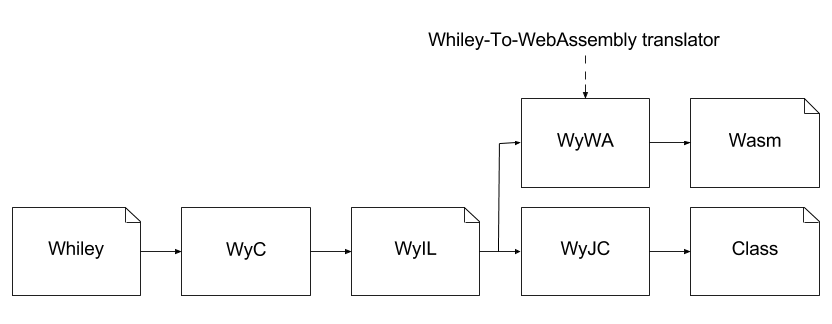
\includegraphics[width=0.8\textwidth]{My_Preposed_Extention}
  \caption{Whiley Compiler Pipeline}
  \label{fig:arc}
\end{figure}

Then a WyIL file is passed to Whiley-to-WebAssembly translator. The translator will construct and output a wasm file. 


\subsection{Design Challenges}\label{subsec:didc}

Throughout this project there have been several important challenges that needed to be overcome. These challenges will be discussed within this section as well as how they were over come. 

\paragraph{}
Conversion of unstructured control flow used by the WyIL files (seen in figure \ref{fig:wyil}) to the structured control flow of Web Assembly and branching, as mentioned in \ref{subsec:wad}, is a challange. The technique that is used is based on how Enscripton transforms LLVM to JavaScript \cite{Zakai:2011:ELC:2048147.2048224}.
%To add more.

\paragraph{}
Also a challenge is the heap and pointers in wasm are addressable memory (the heap) and integers that represent locations in that memory (pointers). The design takes values intended for the heap and assigns them a location. The location is then used to reference them again. 
%Need more consistent nameing sceam.

\paragraph{}
Arrays and records in Whiley, as mentioned in section \ref{subsec:wy} both have value semantics.% Add more detail about what i mean by value semantics.
 The challenge is to ensure that these semantics are not changed when compiled from Whiley to wasm. To ensure this, every time a reference is assigned or used in a method a copy is created. 


\paragraph{}
Finally type information at runtime is important for casting and managing referenced types on the heap. To manage this type information from the WyIL file needs to be stored in wasm. %Add more explination here.


\section{Implementation}

This section covers the implementation of the abstract syntax tree along with the implementation of the design challenges from \ref{subsec:didc}.

\subsection{Abstract Syntax Tree}

The abstract syntax tree (AST) is made to represent wasm as specified in \cite{11_webassembly/spec_2016} and \cite{10_gohman_bastien_wagner_2016}.  This is added to improve the representation of wasm in code. Previously wasm was represented as a string, this creates problems when it comes to code modification. As a result the programs representation became tied in with creation.

\begin{figure}[H]
  \centering
  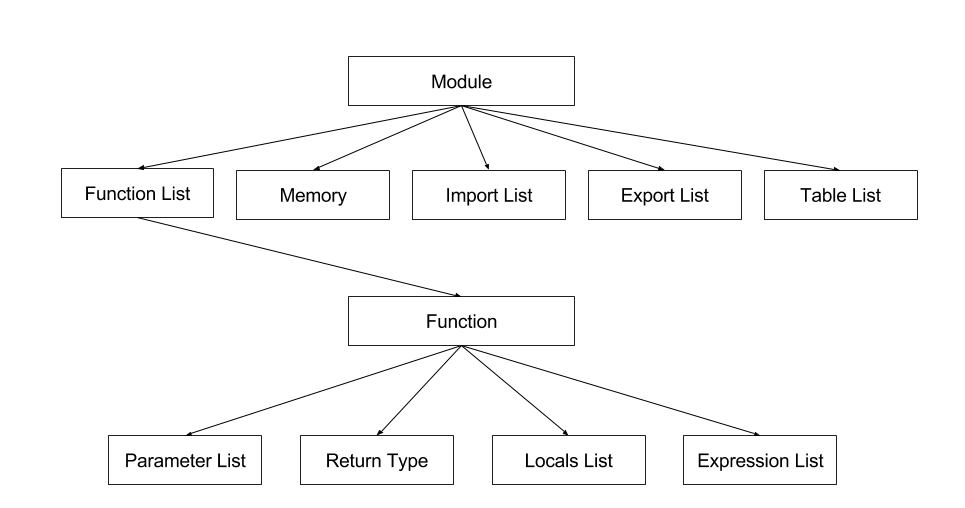
\includegraphics[width=0.8\textwidth]{AST}
  \caption{Simplified Web Assembly AST}
  \label{fig:ast}
\end{figure}

\paragraph{}
Figure \ref{fig:ast}, shows the overall structure of the AST when constructed. Modules the overall structure of the file storing important information like the size of the heap (Memory) and the list of functions defined (Function List). Functions have information about the parameters, locals, return type and expressions that are evaluated within the function. The diagram is missing the large amount of expressions that have been implemented. 

\subsection{Design Challenge Solutions}\label{subsec:didcs}

\paragraph{Unstructured Control Flow}
is transformed into structured control flow using a loop that can loop arbitrarily many times around a large collection of if statements. This transformation can be seen in figure \ref{fig:wtw}. If there are no labels in the WyIL code then Transform 1 will happen regardless. Each transform wraps code within a if statements that checks against the pc value. The pc value is set so that the first statement is always executed. 

\begin{figure}[H]
  \centering
  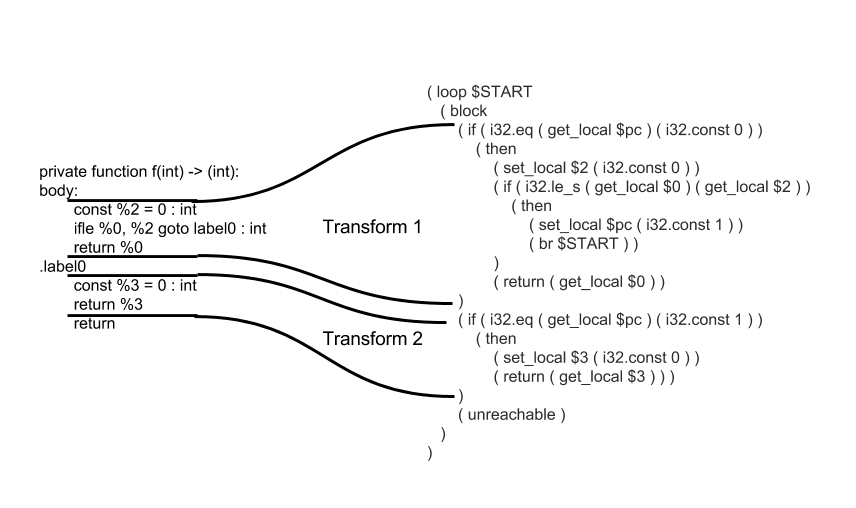
\includegraphics[width=0.8\textwidth]{StatementTransform}
  \caption{WyIL to Web Assembly Transform}
  \label{fig:wtw}
\end{figure}

\paragraph{The Heap and Pointers}
are represented by integers in wasm. This can be seen in figure \ref{fig:hlo}, where the first location on the heap is a pointer to the end and free space. When a new value is added to the heap the base address updates to the new end of heap. This implementation uses a bump pointer and is not efficient because, when memory is no longer needed it cannot be used again. Values that are created and then stored on the heap will keep a reference to the start of that value.

\begin{figure}[H]
  \centering
  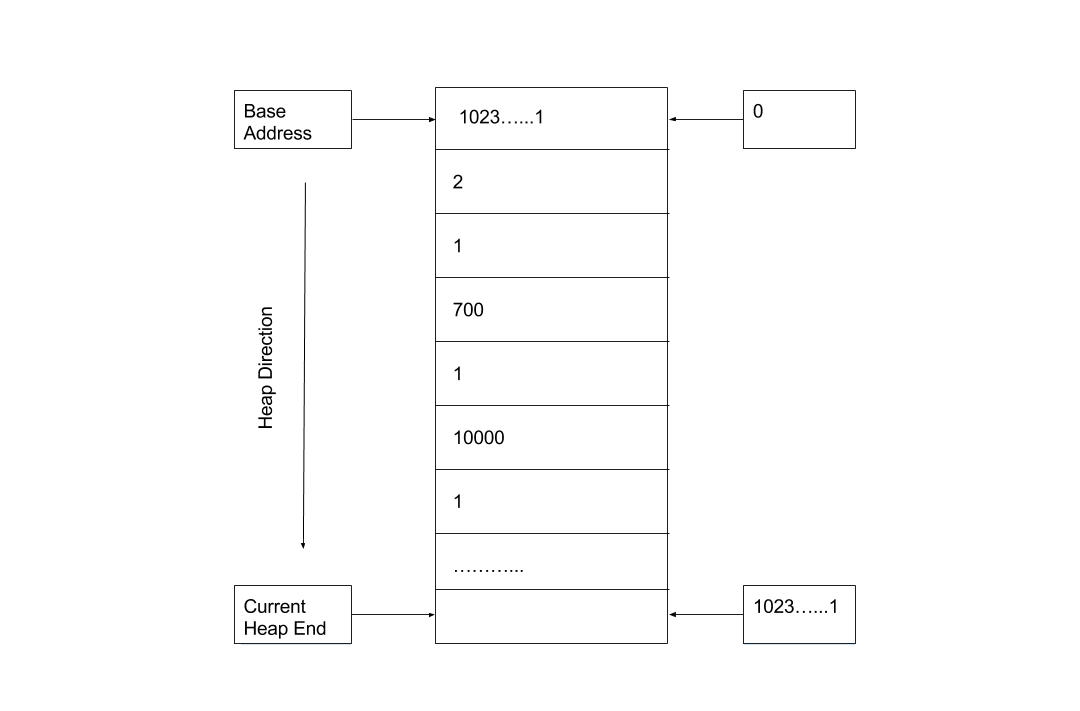
\includegraphics[width=0.8\textwidth]{HeapLayout}
  \caption{Heap Layout}
  \label{fig:hlo}
\end{figure}

%% TODO: Fix this so it is split into two differnet paragraphs.
\paragraph{Arrays and records}
 are stored on the heap in the same structure, see figure \ref{fig:arl}, this allows runtime copying function to be applied to the heap without large amounts of work. This implementation does use more space on the heap but it simplifies memory management.
 
\begin{figure}[H]
  \centering
  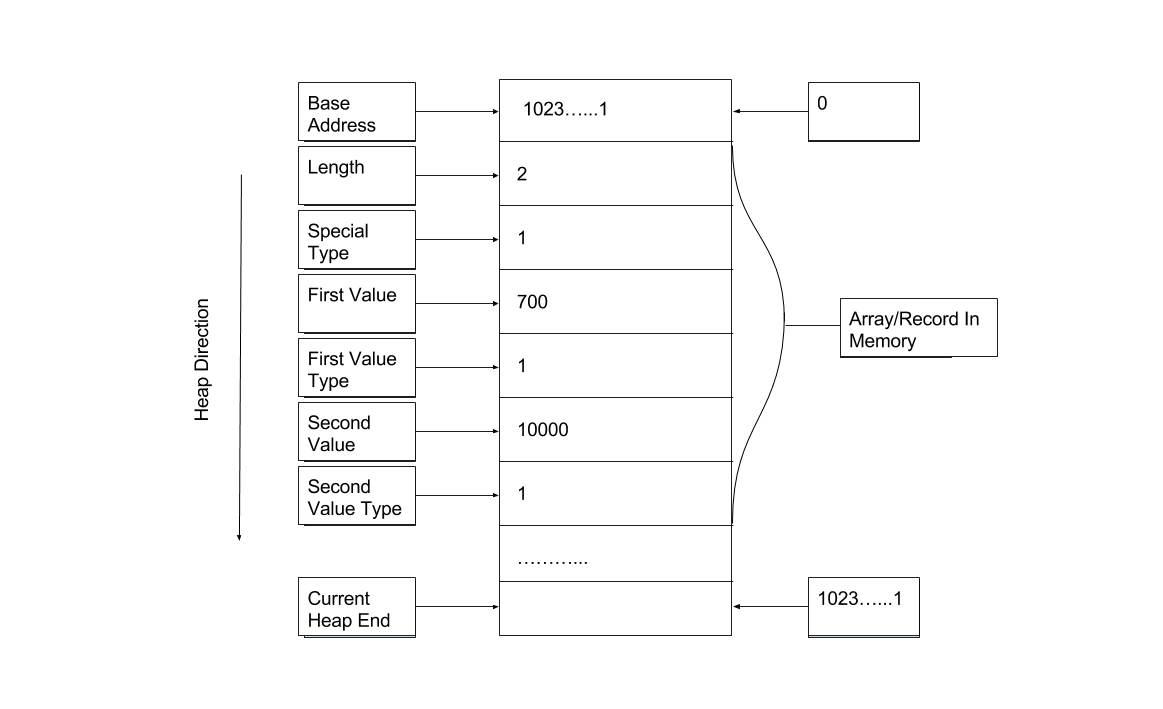
\includegraphics[width=0.8\textwidth]{ArrayLayout}
  \caption{Array and Record Layout on the Heap}
  \label{fig:arl}
\end{figure}

%Cover some information about the runtime copy function.

\paragraph{Type Information}
is stored for each variable and reference as well as values in data structures on the heap as seen in figure \ref{fig:arl}. Each type is mapped to an integer at compile time. This implementation is considered to as a closed world assumption. This means no types from outside the program can be used at runtime this is efficient but limiting. This is efficient because extensive type checking does not need to be made but it does restrict types available to define in the program. Arrays and record type information differs from non referenced values by having their type information in more than one place. The type stored with the reference tells whether it is a array, or a record, nothing else. The structure on the heap seen in figure \ref{fig:arl}, has extra information stored after the length value. For arrays this represents the super-type/type of elements within the array and for records this represents the types and names of fields. 

\chapter{Evaluation}\label{C:t}

This chapter covers the testing framework, what current testing has come up with and the development work flow of the project.

\section{Testing Framework}

The Whiley compiler includes 440 end to end tests. Each tests case consists of a Whiley file that is valid which contain assertions to assert correctness. Each assersion verifies aspects of the Whiley language. Testing of the project is done by loading in the test files and constructing a test case for each file. These files are then run through the Whiley to Web Assembly compilation step with the output of a test.wast file. This file has testing commands appended to it and is then run through the Web Assembly Interpreter. The interpretor confirms correctness of the compiled tests by running append tests commands and outputting a pass result or failure with reasons.%%Cite Interprotor location
The returned value from the interpreter is then used to confirm if the test passed or failed. If the test fails debugging information of failure step is reported to the console. These tests provide a benchmark related to the coverage of the Whiley to Web Assembly compilation step.  

Current testing shows that out of the 440 there is 241 tests passing. The tests that failed have three reasons for failing, that are either unimplemented, bugs, or known features. Each test failure has been looked through and codified and divided up into three overarching failure types with more specific reasons for failure.

\subsection{Unimplemented Functionality}

The amount of test that fail due to unimplemented functionality is the largest section of tests. %%TO ADD. 
Below in Table \ref{fig:table1} you can see the unimplemented functionality and there associated failed tests. 

\begin{figure}[H]
  \centering
  \begin{tabular}{| l || r |}
  \hline
  Null Type & 0 \\ \hline
  Byte Type & 0 \\ \hline
  Lambda & 0 \\ \hline
  References & 0 \\ \hline
  Negation Type & 0 \\ \hline
  Open Record & 0 \\ \hline
  Recursive Type & 0 \\ \hline
  Convert Statement& 0 \\ \hline
  IfIs Statement & 0 \\ 
  \hline
  \end{tabular}
  \caption{Unimplemented functionality and associated test numbers.}
  \label{fig:table1}
\end{figure}

Types not implemented make up most of the failed tests from this subsection. Types such as Null and Byte should be simple to add except for the added complication in the case of Null where it needs to be handled appropriately. %%TODO add example of null in image of handling in if statement.
No effort has been put in to implement lambda functions and recursive types and convert bytecode/casting. Therefore, it remains uncertain how lon git would take to add these features. IsIf bytecode is the runtime type testing bytecode, a simple type system has been added but no effort has been made to make use of it in relation to the IsIf bytecode.  As such it will be difficult to implement IsIF as there is currently no sub-typing explicitly being taken into account. An example of the current typing can be seen %% Link to example.
. 
References should be easy to add in as the underling structure of both Records and Arrays is built on the idea of using references this can be seen in %% Example here.
. %% Todo add explanation of Refrences or link to one.

\subsection{Bugs}

%%Coding ... Testing 

Program errors produce the lest amount of errors although there is possibility of crossover into compiler errors. The Table \ref{fig:table2} (Bellow) shows problems with programming related errors and the amount of tests associated with them.

\begin{figure}[H]
  \centering
  \begin{tabular}{| l || r |}
  \hline
  Number formatting exception & 0 \\ \hline
  Infinite loop & 0\\ \hline
  \hline
  \end{tabular}
  \caption{Program errors and associated test numbers}
  \label{fig:table2}
\end{figure}

Number formatting exception are happening due to the use of "Integer(String)" constructor when getting the type for integers constants. This problem is interesting due to the fact that for most number parsing works fine. Only for a small amount of constants does the problem happen and when it does the string contains numbers as expected, well under the max integer range. This problem requires more investigation to find out the cause.%%Todo add more information about the error. 
Infinite loop happens in only a single test, this test contains open records. This feature is not implemented and for an unknown reason goes into a infinite loop.

\begin{figure}[H]
  \centering
  \caption{Example of a open record}
  \label{fig:table2}
\end{figure}

\subsection{Known Features}
This section contains test that fail with reasons that are known. If statement because it is poorly implemented and Class cast exception because of known unimplemented functionality.

%% Things not fully implemented.
\begin{figure}[H]
  \centering
  \begin{tabular}{| l || r |}
  \hline
  IfEq Bytecode & 0 \\
  Class cast exception & 0 \\ \hline 
  \hline
  \end{tabular}
  \caption{Program errors and associated test numbers}
  \label{fig:table2}
\end{figure}

The IfEq bytecode implementation has the problem where they do not take into account all possible uses. For example when a record contains an array, the implemented IfEq bytecode will not handle the array appropriately. It will look at the contents of the record and compare the pointers of the arrays with each other and not the contents. This is not the intended purpose, step need to be taken to have better handling of both arrays and records. The simplest option is to move array and record checking to a function that is called at run time, or extensive work on the current append in-line method. 
When new objects are made in Whiley and that object is updated at any point in code, a class cast exception will be thrown during compilation. New object are in the case of Whiley are a pointer to a initialized record. They way this is implemented in WyIL uses a different type for updating records or pointers to records and this is not taken into account in the update handling method.  

\section{Results}

\subsection{Benchmarking}

\subsection{Results and Graphs}

\subsection{Result Discussion}



\chapter{Future Work}\label{fw}

\section{Evaluation}

Currently there are three possible ways of evaluating the Whiley-to-WebAssembly translator. The first is to use various benchmarking tools to evaluate the language running with David's pre-made programs in Whiley. The second is to look at the test suite and look at the number of tests that are passing for what reason. For those that are failing, look at why they are failing. Last do a comparison of both Whiley-to-WebAssembly and Whiley-to-JavaScript is required. Whiley-to-JavaScript was made last year as an honors project (cite whose). A comparison of the two will show important differences between JavaScript and Web Assembly, while noting that implementation of compiler must be taken into account.

\section{Functionality}

Functionality that is still required in the compiler step is as follows. 

\paragraph{}
More work needs to be done on reference types. The reference types are currently unable to access reference. Update has a similar issue.  Deep copying has a function for handling this but it is not used in all required places. Mixing of access between arrays and records accesses needs work as well. 

\paragraph{}
WyIL operations need to be implemented such as Array Generators and Quantify statements. Along with those is the requirement for reference semantics and byte types to be implemented. The time required to do all of the above implementations, should not be long as they are based on other work or in the case of reference semantics the removal of previous work in this special case.

\paragraph{}
Type checking still needs to be implemented. There is currently a way of checking the type of any variable as mentioned in \ref{subsec:didcs}. Cast and ifis statements are not implemented, this is the first step in being able to implement Whiley's union types. More work also needs to be put in around handling subtyping based on the information from the implemented type system.

\section{Performance Improvements}

Performance can be improved by implementing the following improvements.

\paragraph{}
Reference counting can be used for improving memory management above its current capabilities. This is because each reference variable needs to point to a different place in memory. This includes when no modification will ever be made to the reference location of both the copied and original memory. If reference counting was used, the copying of memory would be put off until the point when modification is planned. The reference counter would be checked, if it was larger than one, then decrease the counter, copy the memory, then modify, otherwise just modify.






%%%%%%%%%%%%%%%%%%%%%%%%%%%%%%%%%%%%%%%%%%%%%%%%%%%%%%%

\backmatter

%%%%%%%%%%%%%%%%%%%%%%%%%%%%%%%%%%%%%%%%%%%%%%%%%%%%%%%


%\bibliographystyle{ieeetr}
\bibliographystyle{acm}
\bibliography{eng}



\end{document}
